\chapter{Introduction of the Task Scheduling Problem}
In modern era, with the development of artificial intelligent and machine learning technology, robots are becoming deeply integrated into people's life. Therefore, robot path planning is a hot topic that attacks a lot of scientists attention. Among all these robot path planning problems, due to the wide potential of application, \textbf{task scheduling} is one of the most famous question that that has been under debate for long time. There are many versions of problem statement for this task scheduling problem, but one of the most basic and fundamental format is stated as the following: 
\section{Problem Statement}
Assume there are K homogeneous robots and M targets randomly distributed in a bounded 2D space. Each target requires \textbf{at least one} robot, and each of the robots need to be assigned to one target (in this basic format, we are not considering the situation where one robot can do multiply tasks). This is to say, the task assignment, $f$ , is a map on $\mathbf{R^2}$ from set $\mathbf{Robots}$ to set $\mathbf{Tasks}$. 
\begin{equation}
    f:{\mathbf{Robots}} \to \mathbf{Tasks}
\end{equation}
The cost function, $C$, is defined as the summation of robots' travelling path from their origin to their assigned tasks:
\begin{equation}
   C = \sum\limits_{{\rm{robots}}} {{\rm{Path\quad } \rm{Length}}} 
\end{equation}
\\
The challenge is to develop a good algorithm to find a traveling path for all the robots with the minimum or near minimal cost.
\\
A visual illustration is given as shown in the picture \ref{fig:birds}, all the M green squares are tasks (in this case, $M=5$, and tasks are labeled as $T_0$ to $T_4$) need to be accomplished, and all the K red dots are robots (in this case, $K=8$, and robots are labeled as $R_0$ to $R_8$) that need to be assigned for a task. All the initial position for tasks and robots are randomly generated in the range of $[0,5]$, and the arrangement with the lowest cost is la-bled with red lines which are generate from a \href{https://github.com/ENGG6570/Group-Project/tree/main/ENGG6570_Project}{Python brute-force program}  . 

\begin{figure}[h!]
  \centering
  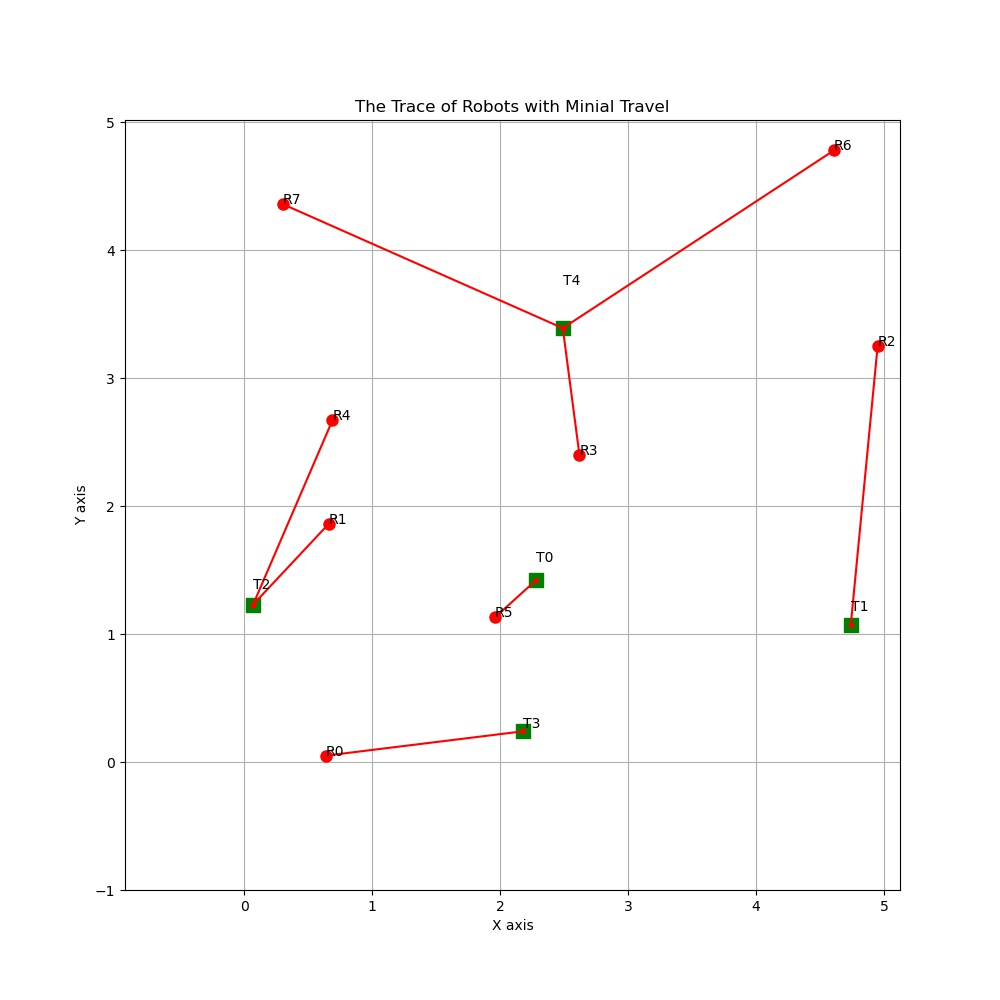
\includegraphics[width=15cm]{Pictures/ProblemStatement.jpeg}
  \caption{The illustration of Task Scheduling Problem with 5 tasks and 8 robots.}
  \label{fig:birds}
  \Description{}
\end{figure}

\section{The Brute-force Method}
Theoretically, at small scale, we can solve this problem and find the best solution with the Brute-force method. The time complexity will be bound by $O(M^K)$. Same as the famous traveling sales person (TSP) problem, this is a NP-complete problem as well.
\subsection{Entropy of this problem}
\\ According to Shannon's information theory\cite{Shannon1948}, for a random variable $X$ in a finite set $\chi$ with probability distribution $p(x)$ , the  Shannon's entropy can be written as:
\begin{equation}
    H\left( X \right) =  - \sum\limits_{x \in \chi } {p\left( x \right){{\log }_2}\left( {p\left( x \right)} \right)}\label{shannon}
\end{equation}
For each of the robots, it will have at most M choice to choose from as its the target. The total number of possible of arrangement is at most $M^K$. With considering the boundary condition that each of these M target need to have at least one robot, we can reduce the total number of possible of arrangement, $\chi$, as: 

\begin{equation}
\begin{array}{*{20}{c}}
\chi & = &{\underbrace {M\left( {M - 1} \right)\left( {M - 2} \right) \ldots 1}_{M!} \times C_{K - M}^K{M^{K - M}}}\\
{}& = &{M!\frac{{K!}}{{\left( {K - K + M} \right)!\left( {K - M} \right)!}}{M^{K - M}}}\\
{}& = &{\frac{{K!}}{{\left( {K - M} \right)!}}{M^{K - M}}}
\end{array}
\end{equation}

\subsection{Time Analysis and Entropy Analysis}
With a home used i7-9700K CPU (8 Cores, 3.6GHz), the maximum scale size of this problem that can be solved without memory leaking is 2 tasks and 20 robots (See Figure \ref{fig:upperlimit}), or, 8 robots and 8 tasks. Table \ref{tab:bruteforce} is a summaries the time complexity of this problem with the Brute-force method:

\begin{table}[]
    \centering
\begin{tabular}{|l|l|l|l|l|}
\hline
M & K  & Time     & $\chi$       & $H(\chi)$ \\ \hline
2 & 2  & 0.0005   & 2       &  1.000 \\ \hline
2 & 4  & 0.0005   & 14      &  3.807 \\ \hline
2 & 8  & 0.001488 & 254     &  7.988 \\ \hline
2 & 16 & 0.65571  & 65534   &  15.999 \\ \hline
2 & 20 & 13.02    & 1048574 &   20.000\\ \hline
\end{tabular}
    \caption{The time complexity analysis of this problem with 2 tasks, and $K = 2^n$ robots}
    \label{tab:bruteforce}
\end{table}

\begin{figure}[h!]
  \centering
  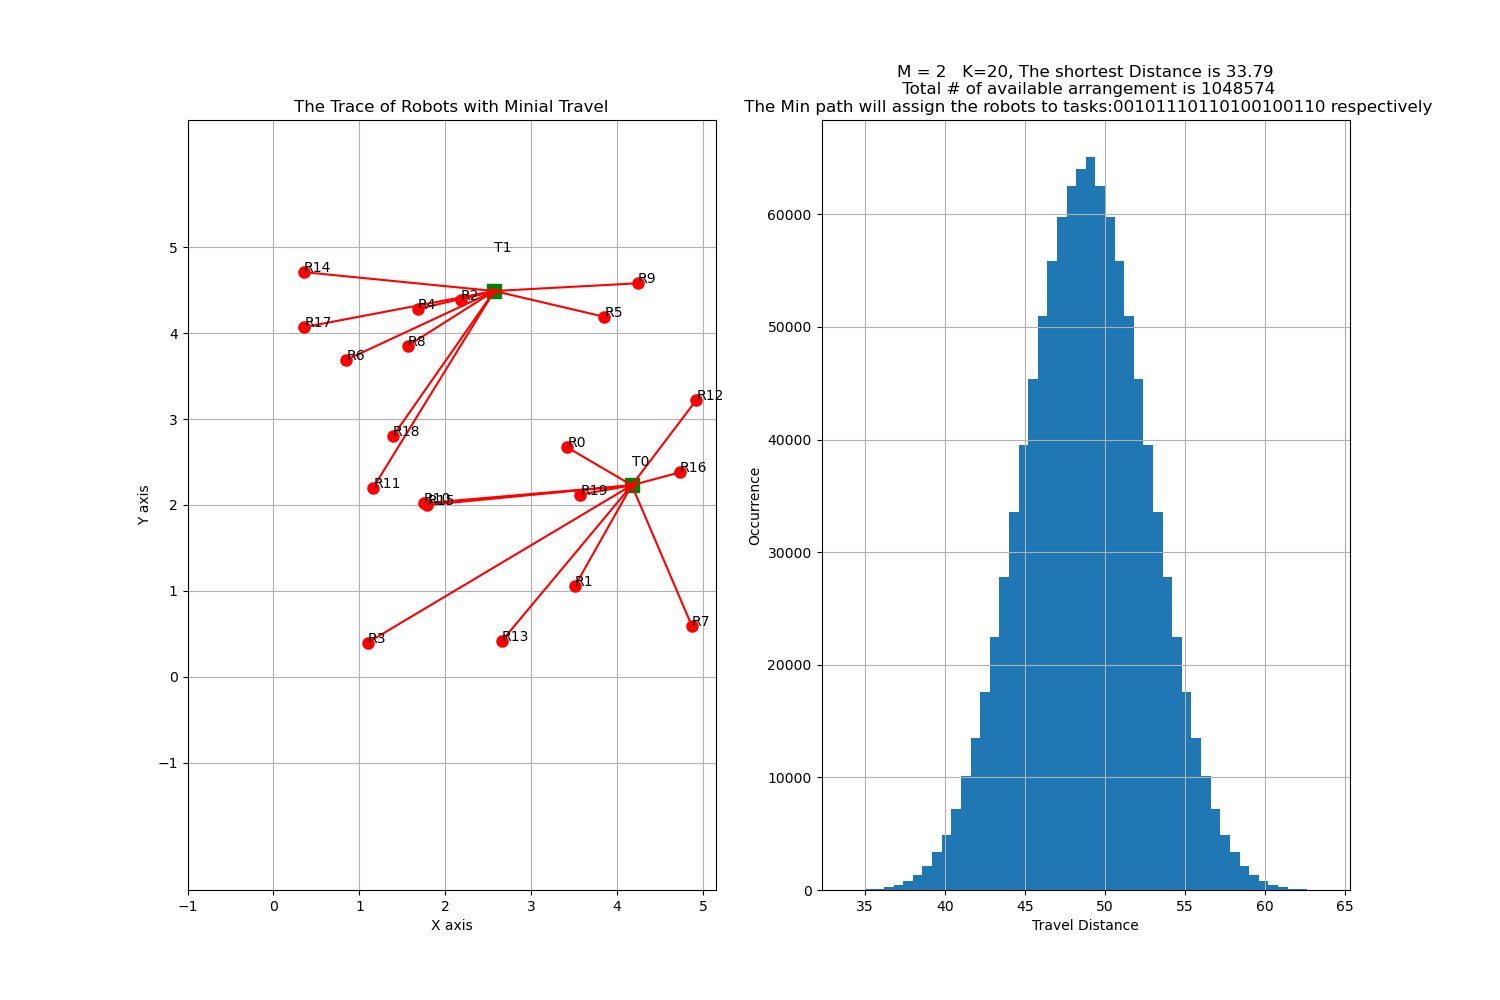
\includegraphics[width=15cm]{Pictures/220.png}
  \caption{The maximum scale size of this problem that can be solved on a PC is 2 tasks and 20 robots}
  \label{fig:upperlimit}
  \Description{}
\end{figure}